\documentclass{article}
\usepackage[T1]{fontenc}
\usepackage{graphicx}
\usepackage{lipsum}
\usepackage{float}
\usepackage{amsmath}
\usepackage[hidelniks]{hyperref}
\subsection*{Exercise 4: Float Placement with Different Specifiers}
\begin{document}
\lipsum[1-2]

\begin{figure}[h]
    \centering
    
\includegraphics[width=0.4\textwidth]{example-image-a}
    \caption{Option h (here)}
    \label{fig:h}
\end{figure}

\lipsum[3]
\begin{figure}[t]
    \centering
    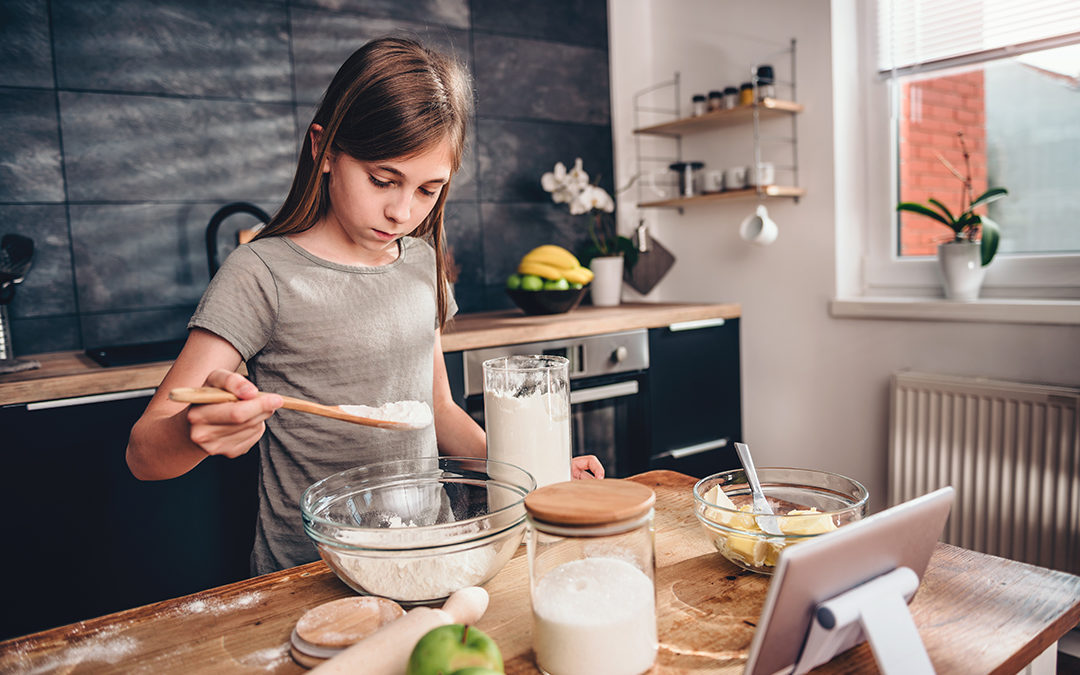
\includegraphics[width=0.4\textwidth]{example-image-b}
    \caption{Option t (top)}
    \label{fig:t}
\end{figure}

\begin{figure}[b]
    \centering
    
\includegraphics[width=0.4\textwidth]{example-image-c}
    \caption{Option b (bottom)}
    \label{fig:b}
\end{figure}

\lipsum[4-8]
\textbf{Observed interactions:}
\begin{itemize}
\item \texttt{[h]} : Tries to place the float at the exact location
\item \texttt{[t]} : Priority for top of page
\item \texttt{[b]} : Priority for bottom of page
\item \texttt{[ht]} : Combines "here" and "top" possibilities
\item The more options you add, the more flexibility LaTeX has for placement
\end{itemize}
\end{document}

